%% document class
\documentclass[10pt]{beamer}
%%theme
\usetheme[hideothersubsections,width=2cm]{Berkeley}
%% page settings
\usepackage{xcolor}
\usenavigationsymbolstemplate{}
\usefonttheme{serif}

%% packages
\usepackage{courier}
\usepackage{geometry}
\usepackage{graphicx}
\usepackage[scaled=0.9]{helvet}
\usepackage{multimedia}
\usepackage{mathptmx}
\usepackage{tikz}
\usepackage{xmpmulti}

%%color settings
%%%%% Color Schema

\definecolor{blue_dark}{RGB}{38,50,56}
\definecolor{blue}{RGB}{33,150,243}
\definecolor{blue_light}{RGB}{79,195,247}
\definecolor{grey_dark}{RGB}{38,50,56}
\definecolor{grey}{RGB}{33,150,243}
\definecolor{grey_light}{RGB}{33,150,243}

%% theme settings
\setbeamercolor*{palette primary}{fg=grey_dark,bg=blue_light} % upper part
\setbeamercolor*{palette secondary}{fg=grey_dark,bg=blue_light} % left part (background)
\setbeamercolor*{sidebar left}{fg=blue_light,bg=grey_dark} % left part with links
\setbeamercolor*{palette sidebar primary}{fg=blue_light}
\setbeamercolor*{palette sidebar secondary}{fg=blue_light}
\setbeamerfont{section in sidebar}{size=\scriptsize}

%% new commands
%\input{settings/macros}
\addtobeamertemplate{frametitle}{\vskip+0.6ex}{}
\makeatletter
\beamer@headheight=2\baselineskip
\makeatother

\begin{document}

\author[Group 9]{Suvojit Manna\\Pronab Mukherjee\\Barun Gupta\\Somnath Rakshit\\}
\title[Machine Learning]{Introduction to Machine Learning using \LaTeX}
%\logo{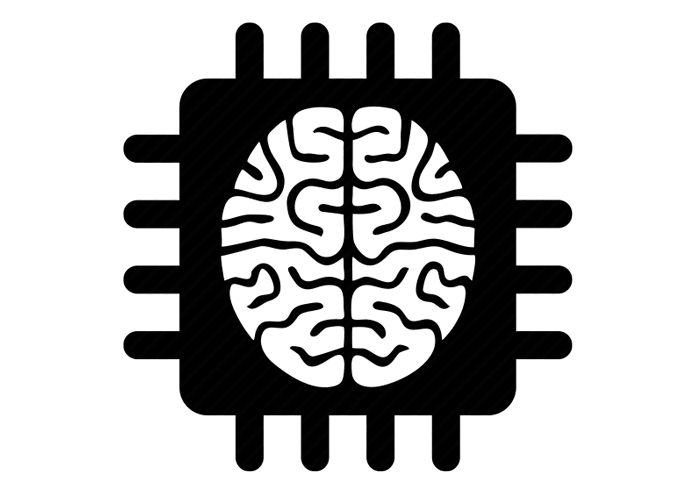
\includegraphics[width=4mm]{images/icon}}
\institute[JGEC]{Jalpaiguri Govt Engineering College}
%\date{City, date}


%% Title Page
\begingroup
\setbeamercolor{background canvas}{bg=blue_dark}
\begin{frame}[plain,t]
	\hspace*{-22 mm}
	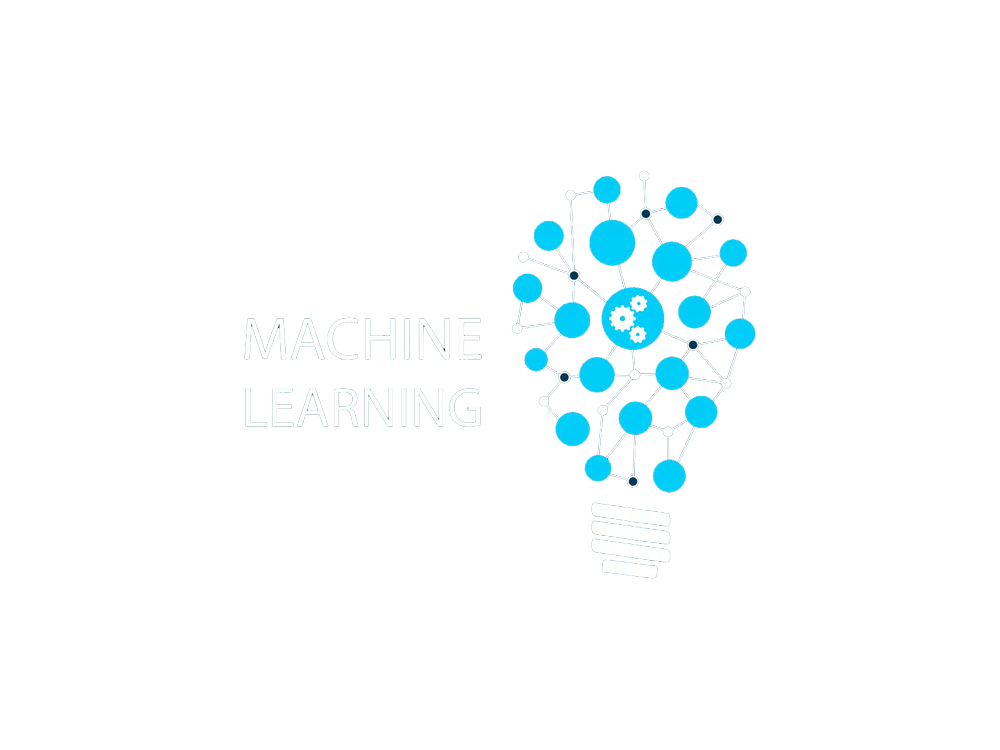
\includegraphics[width=\paperwidth,height=\paperheight]{images/ml_bg}
\end{frame}
\endgroup

%% A Team Page
\begingroup
	\usebackgroundtemplate{%
		\tikz\node[opacity=0.3] {
\includegraphics[height=\paperheight,width=\paperwidth]{images/bg-vec}}
		;}
	\begin{frame}[c]{The A Team}
		\begin{center}
			\Huge{Presented By:\\}
			\large{~\\Suvojit Manna\\Pronab Mukherjee\\Barun Gupta\\Somnath Rakshit\\}
		\end{center}
	\end{frame}
	%% contents
	\begin{frame}{Contents in Brief}
		%\tableofcontents
		\tableofcontents[hideallsubsections]
	\end{frame}
\endgroup
	%% Big Font Page: Lets get started
\begingroup
	\setbeamercolor{background canvas}{bg=blue_dark}
	\setbeamercolor{normal text}{fg=blue_light}
	\begin{frame}[plain,c]
		\hspace*{10 mm}
		\vspace*{-18 mm}
		\textcolor{blue_light}{\Huge{Let's Get Started}}
	\end{frame}
\endgroup


\begingroup
	\usebackgroundtemplate{%
		\tikz\node[opacity=0.3] {
\includegraphics[height=\paperheight,width=\paperwidth]{images/bg-vec}}
		;}
	
	\section{Introduction}
		\begin{frame}{Machine Learning | What ?}
			\begin{center}
				\large{Field of study that gives computers the ability to learn without being explicitly programmed.}\\
				\bigskip
				\small{Instead of writing code, you feed data to the generic algorithm and it builds its own logic based on the data.}
				\begin{figure}
				\centering
				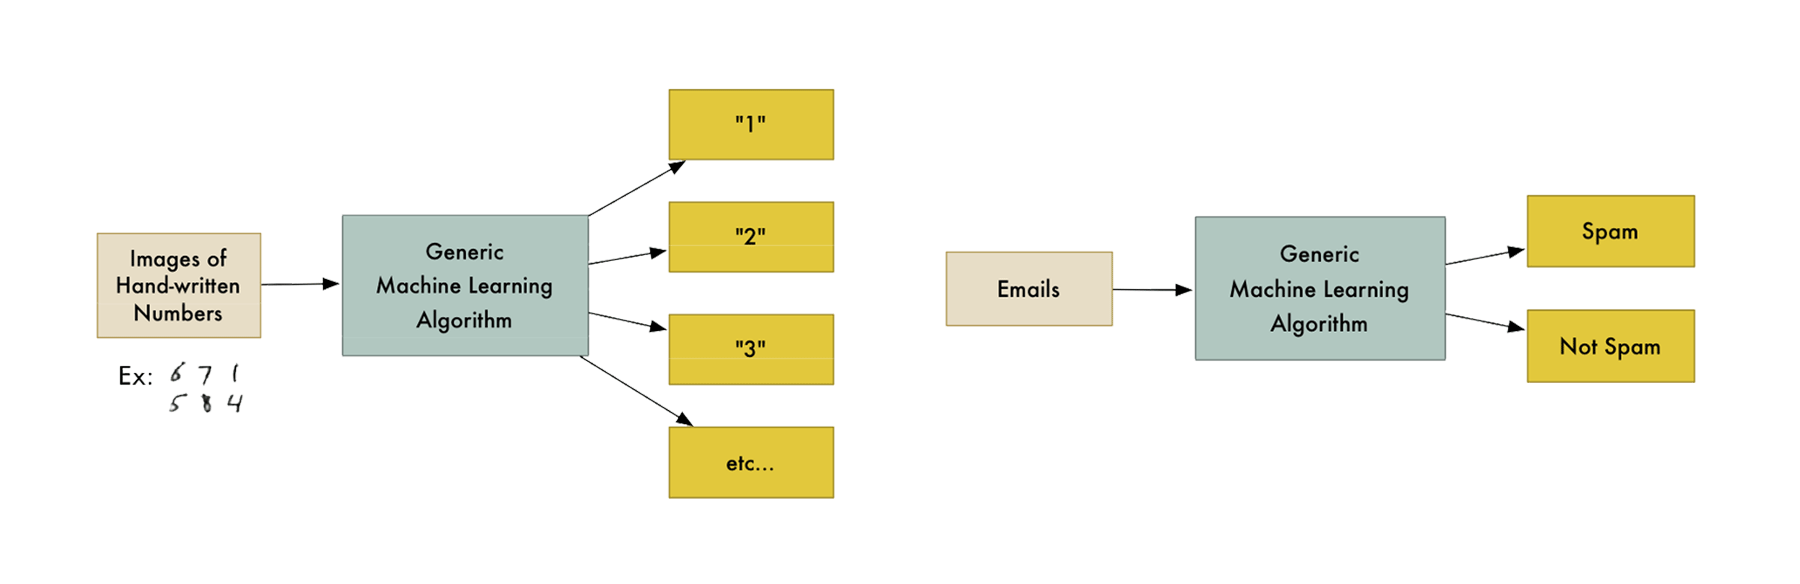
\includegraphics[width=\linewidth,height=30mm]{images/classif-ex}
				\caption[This machine learning algorithm is a black box that can be re-used for lots of different classification problems.]{Classification Algorithms}
				\end{figure}
			\end{center}
		\end{frame}
		\subsection{Case Studies}
			\begin{frame}{Case Studies | Supervised Learning}
				\begin{center}
					\begin{tabular}{|c|c|c|c|}							\hline 
						\bfseries{Bedroom} & \bfseries{Sq.Ft} & \bfseries{Neighbourhood} & \bfseries{Price}\\ 	\hline
						3       & 2000  & Uptown        & \$350,000 \\ 	\hline 
						2       & 800   & Downtown      & \$200,000 \\ 	\hline 
						2       & 850   & City Centre   & \$150,000 \\ 	\hline 
						1       & 550   & Suburbs       & \$75,000 \\	\hline 
						4       & 2000  & Suburbs       & \$200,000 \\	\hline 
					\end{tabular}\\
					\bigskip
					\begin{tabular}{|c|c|c|c|}							\hline 
						\bfseries{Bedroom} & \bfseries{Sq.Ft} & \bfseries{Neighbourhood} & \bfseries{Price}\\ 	\hline
						3   	& 2000  & City Centre   & ???\\			\hline 
					\end{tabular} \\
					\bigskip
					\begin{block}{Definiton}
						Supervised learning is the machine learning task of inferring a function from labeled training data.
					\end{block}
				\end{center} 
			\end{frame}
			\begin{frame}{Case Studies | Supervised Learning}
				\begin{center}
					\begin{tabular}{|l l|}\hline 
						\multicolumn{2}{|c|}{\textbf{Math's Exam - Answer Keys}}\\
						1) 2  4  5 = 3 & 5) 6  2  2 = 10 \\ 
						2) 5  2  8 = 2 & 6) 3  1  1 = 2  \\ 
						3) 2  2  1 = 3 & 7) 5  3  4 = 11 \\ 
						4) 2  2  4 = 6 & 8) 1  8  1 = 7  \\ \hline
					\end{tabular}\\
					\bigskip
					\begin{itemize}
						\item The training data consist of a set of training examples.
						\item Training Data :
							\begin{itemize}
								\item Input Object : Set of Features
								\item Desired Output : Supervisory Signal
							\end{itemize}
						\item A supervised learning algorithm produces an inferred function.
						\item An analogus task in human and animal phsycology : Concept Learning.
					\end{itemize}
				\end{center}
			\end{frame}
			\begin{frame}{Case Studies | Unsupervised Learning}
				\begin{center}
					\begin{figure}
					\centering
					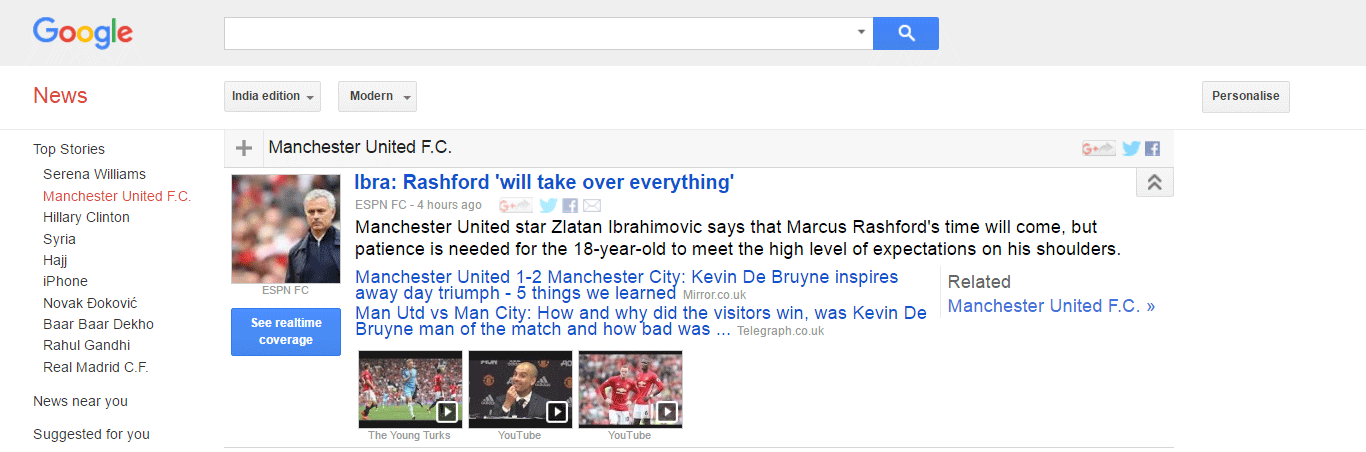
\includegraphics[width=\linewidth]{images/unsupl-ex}
					\caption{Google News grouping similar stories together.}
					\end{figure}
					\begin{block}{Definiton}
						Unsupervised learning is the machine learning task of inferring a function to describe hidden structure from unlabeled data.
					\end{block}
				\end{center}
			\end{frame}
			\begin{frame}{Cocktail Party Problem | Unsupervised Learning}
				\begin{columns}
					\begin{column}{0.5\textwidth}
						Sound from :
						\begin{itemize}
							\item \movie{{\it Microphone 1}}{sounds/cpp-mix1.wav}
							\item \movie{{\it Microphone 2}}{sounds/cpp-mix2.wav}
						\end{itemize}
						\bigskip
						Output from Learning Algorithm :
						\begin{itemize}
							\item \movie{{\it Output 1}}{sounds/cpp-output1.wav}
							\item \movie{{\it Output 2}}{sounds/cpp-output2.wav}
						\end{itemize}
					\end{column}
					\begin{column}{0.5\textwidth}
						\begin{figure}
							\centering
							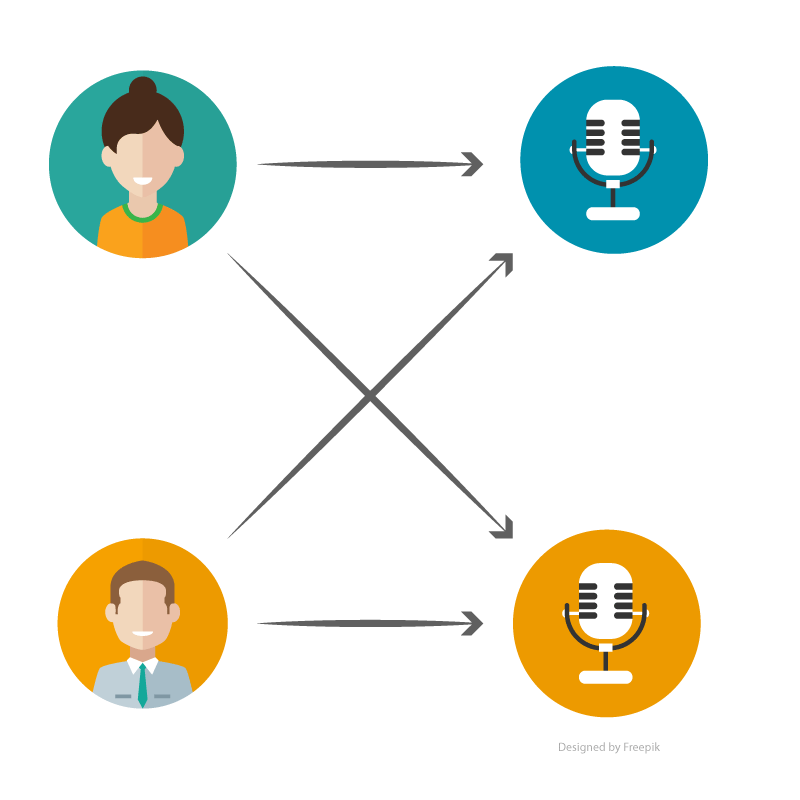
\includegraphics[width=1.0\linewidth]{images/cpp-repr}
							\caption{Overlapped Recordings}
						\end{figure}
					\end{column}
				\end{columns}
			\end{frame}
			\begin{frame}{Case Studies | Unsupervised Learning}
				\begin{center}
					\begin{figure}
						\centering
						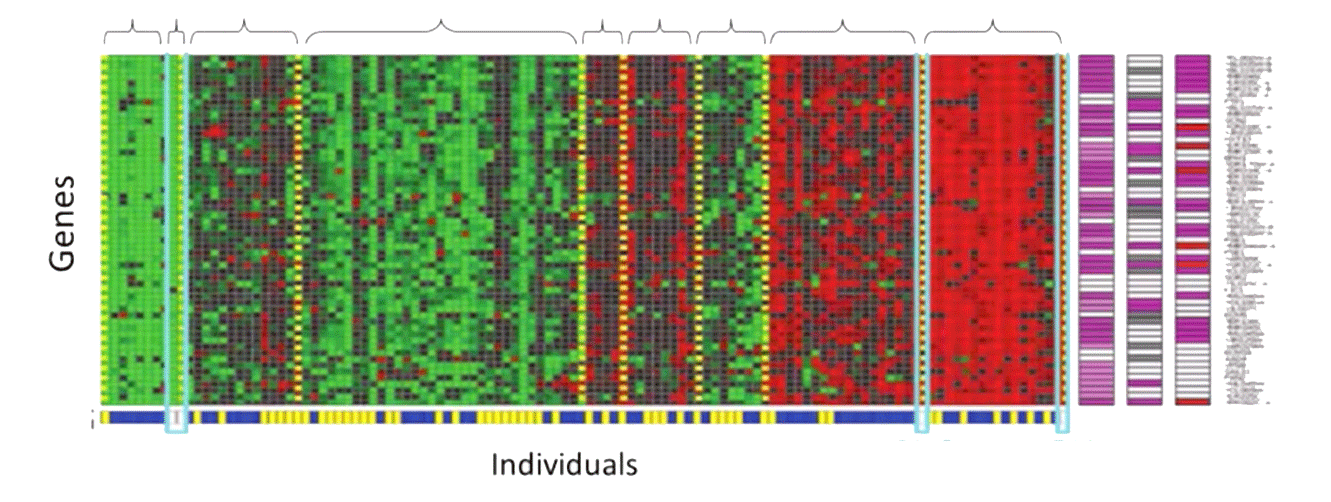
\includegraphics[width=\linewidth]{images/gene-classification}
						\caption[Gene Clustering]{Gene Clustering}
					\end{figure}
					\begin{itemize}
						\item Training Data given to the learner is unlabeled.
						\item No error or reward signal to evaluate a potential solution.
						\item Closely related to density estimation in statistics.
					\end{itemize}
				\end{center}
			\end{frame}
		\subsection{Formal Defintion}
			\begin{frame}{Machine Learning | Formal Definiton}
				\begin{center}
					\small{The field of machine learning is concerned with the question of how to construct computer programs that automatically improve with experience.}\\
					\bigskip
					\large{A computer program is said to learn from experience E with respect to some class of tasks T and performance measure P, if its performance at tasks in T, as measured by P, improves with experience E.}\\
					\bigskip
					\small{Evolved from :}
					\begin{itemize}
						\item {\small Pattern Recognition}
						\item {\small Computational Learning Theory}
						\item {\small Artificial Intelligence}
					\end{itemize}
				\end{center}
			\end{frame}
		\subsection{Applications}
			\begin{frame}{Industry Trends}
				\begin{columns}
					\begin{column}{0.5\textwidth}
						\begin{center}
						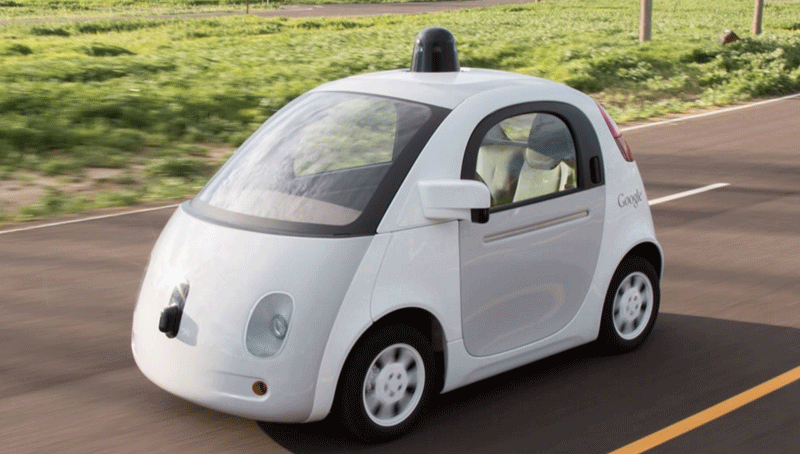
\includegraphics[width=0.9\linewidth]{images/app-2}
						\end{center}
					\end{column}
					\begin{column}{0.5\textwidth}
						\begin{center}
							Google Chauffer :
						Self Driving Car by Google
						\end{center}
					\end{column}
				\end{columns}
				\begin{columns}
					\begin{column}{0.5\textwidth}
						\begin{center}
							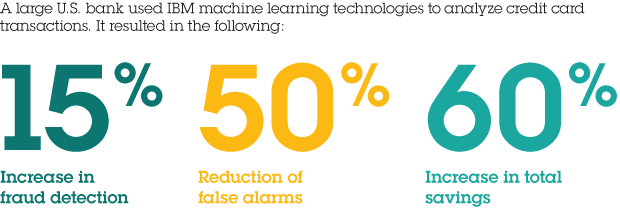
\includegraphics[width=0.9\linewidth]{images/app-3}
						\end{center}
					\end{column}
					\begin{column}{0.5\textwidth}
						\begin{center}
							IBM Research : Credit Card Fraud Detection
						\end{center}
					\end{column}
				\end{columns}
				\begin{columns}
					\begin{column}{0.5\textwidth}
						\begin{center}
							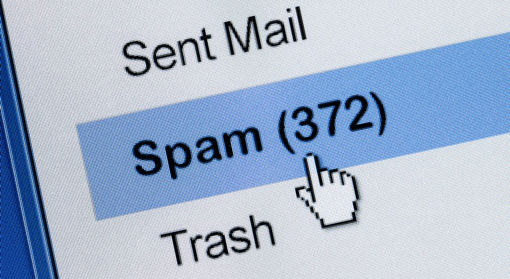
\includegraphics[width=0.9\linewidth]{images/app-5}
						\end{center}
					\end{column}
					\begin{column}{0.5\textwidth}
						\begin{center}
							Mail Services : Spam Filtering
						\end{center}
					\end{column}
				\end{columns}
			\end{frame}
			\begin{frame}{Industry Trends}
				\begin{figure}
					\centering
					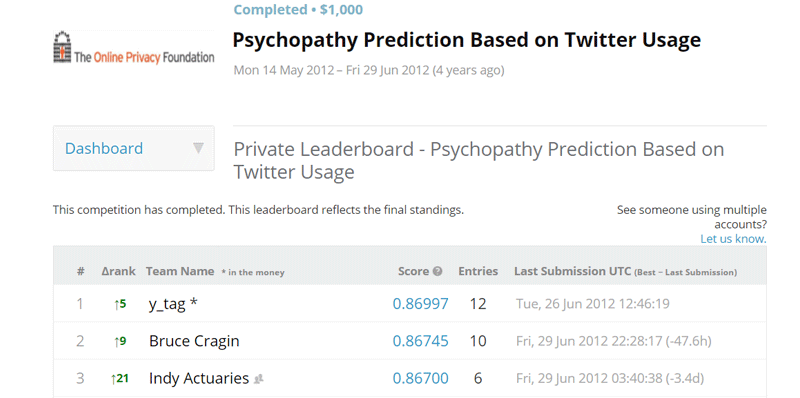
\includegraphics[width=0.9\linewidth]{images/app-1}
					\caption{Kaggle Challenge : Psychopathy Prediction}
				\end{figure}
				\begin{center}
					The  aim of the competition is to determine to what degree it's possible to predict people with a sufficiently high degree of Psychopathy based on Twitter usage and Linguistic Inquiry.
				\end{center}
			\end{frame}
			\begin{frame}{Entertainment | Machine Learning}
				%TODO : Insert MarI/O video
				\movie{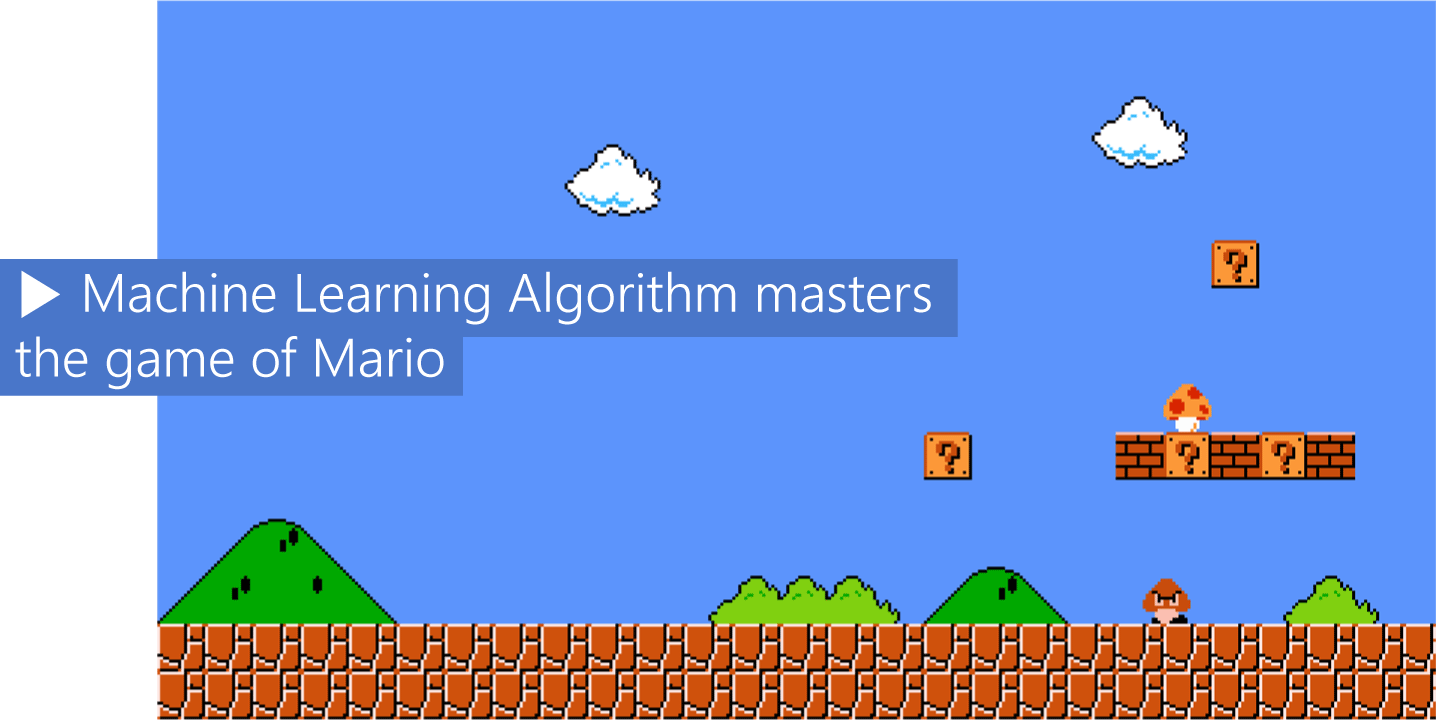
\includegraphics[width=\textwidth]{images/app-6.png}}{video/mario-ml.mov}
			\end{frame}
			\begin{frame}{Applications | Machine Learning}
				\begin{columns}
					\begin{column}{0.5\textwidth}
						\begin{itemize}
							\item Adaptive websites
							\item Classifying DNA sequences
							\item Computer vision
							\item Internet fraud detection
							\item Natural language processing
						\end{itemize}
					\end{column}
					\begin{column}{0.5\textwidth}
						\begin{itemize}
							\item Online advertising
							\item Recommender systems
							\item Search engines
							\item Sentiment analysis
							\item Speech and handwriting recognition
						\end{itemize}
					\end{column}
				\end{columns}
				%TODO : Insert Animation	
			\end{frame}
	\section{Regression}
	\subsection{Introduction}
	\begin{frame}[c]{Regression | What?}
		\begin{center}
			\huge{Regression}
			\Large{ is an}
			\huge{analysis process}
			\Large{ to predict the value of an attribute derived from}
			\huge{ multiple known attributes.}
		\end{center}
	\end{frame}
	
	\begin{frame}[c]{Regression | The Commander of Examples}
		\begin{center}
			\normalsize{Suppose a Commander needs to be chosen out of a bunch of soldiers. Now no such attribute is known which determines the }
			\large{the potential to become the Commander.}
			\normalsize{ \\But other independent attributes are known such as}
			\large{Attendence, IQ Scores, Physical Fitness, Supervisor Rating.}
			\pause		
			\normalsize{\\~\\This is where}
			\Large{ Regression Analysis}
			\normalsize{ comes handy.}
		\end{center}
	\end{frame}
	
	\begin{frame}[t]{Regression | How to?}
		\begin{center}
			\small{First the known attributes are plotted separately. Then a composite plot is aquired from all the separate 						plots. Then we must aquire the
			}
			\large{Regression Line}
			\small{ that is a line that fits the best with all the plots}
			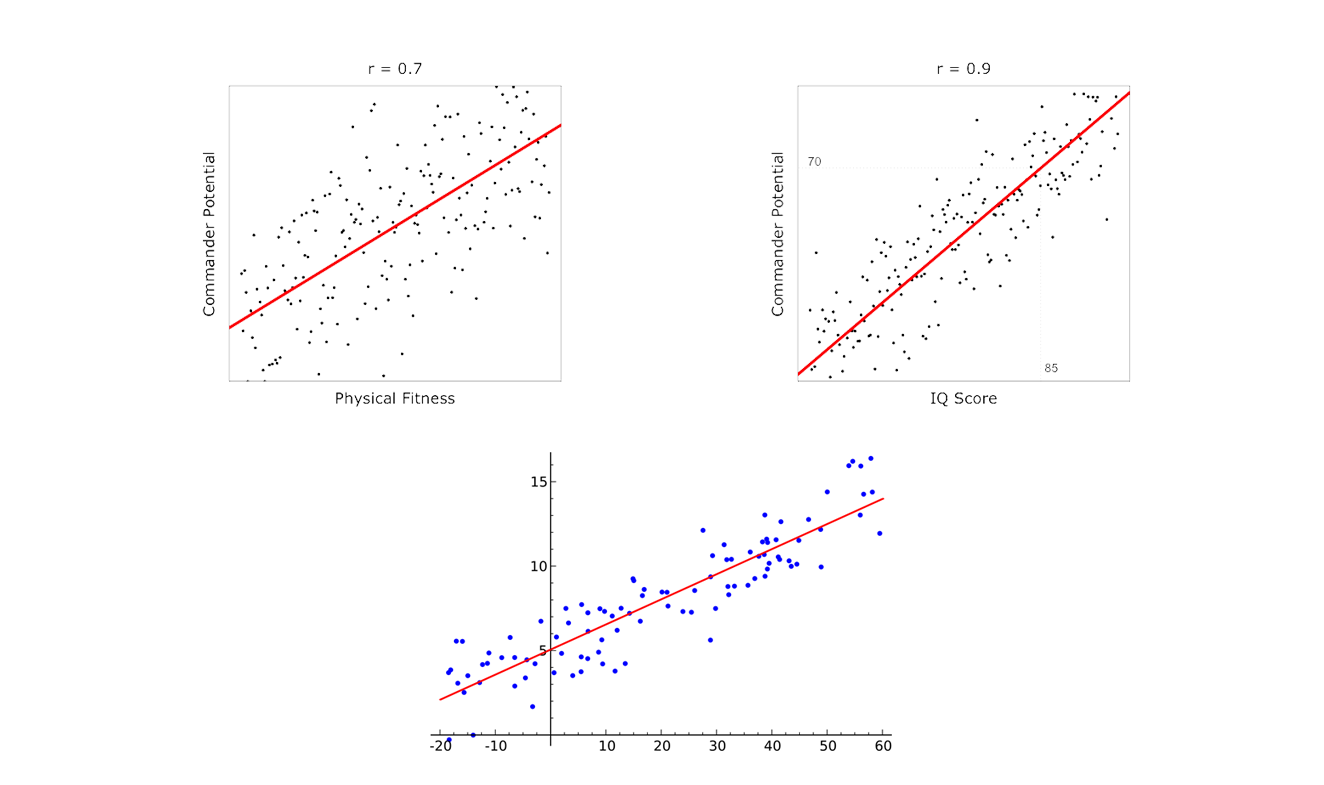
\includegraphics[scale=0.2]{images/ex}			
		\end{center}
	\end{frame}
	
	\begin{frame}[c]{Regression | Formal Definition}
		\begin{center}
			\large{In statistics,}
			\Large{ Regression Analysis}\large{ is a statistical process for estimating the relationships among variables. It includes many techniques for modeling and analyzing several variables, when the focus is on the relationship between a dependent variable and one or more independent variables.
			}
		\end{center}
	\end{frame}
	
	\begin{frame}[c]{Regression | Types of Regression}
		\begin{figure}
			\begin{center}
				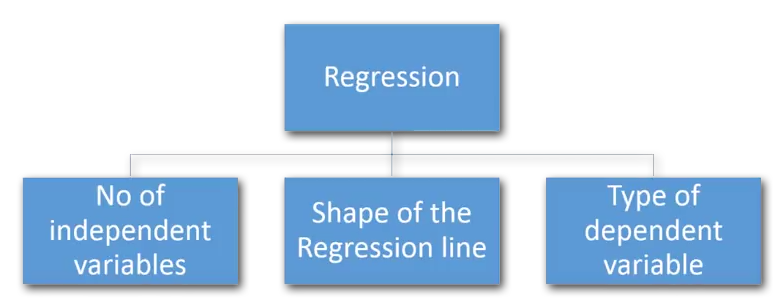
\includegraphics[scale=0.35]{images/regt}
			\end{center}
			\caption{Types of Regression}
		\end{figure}
	\end{frame}
	
	\begin{frame}[c]{Regression | Importance of Regression Line}
		\begin{center}
			\transduration<0-7>{0}
			\multiinclude[<+->][format=png, graphics={width=0.5\textwidth}]{images/tmp}
		\end{center}
	\end{frame}
	
	\subsection{Benefits}
	\begin{frame}{Regression | It's Beneficial }
		\Large{}
		\begin{itemize}
			\setbeamercovered{transparent}
			\item<1-> Estimates Future with minimal error
			\item<2-> Provides Aid in Decision Making
			\item<3-> Self Developing
			\item<4-> Increasing Accuracy
			\item<5-> Develops Big Data and Data Mining   
		\end{itemize}	
	\end{frame}
	
	\subsection{Usages}
	\begin{frame}{Regression | There must be its Uses }
		\Large{Regression analysis}\large{ is most commonly used in}\Large{ forecasting or predicting}\large{ how a set of conditions will impact an outcome.\\~\\}
		\normalsize{\begin{itemize}
				\setbeamercovered{transparent}	
				\item<1> Weather Forecasting
				\item<2> Stock Market Estimation
				\item<3> Statistical Research 
				\item<4> Business Forecasting and Optimization
				\item<5> Risk Forecasting in Medical Fields
				\item<6> Decision Making of Regular Jobs 
			\end{itemize}
		}
	\end{frame}
	
	\subsection{Example Cases}
	\begin{frame}{Regression | Some Real Life Examples}
		\begin{center}
			\vspace{-5mm}
			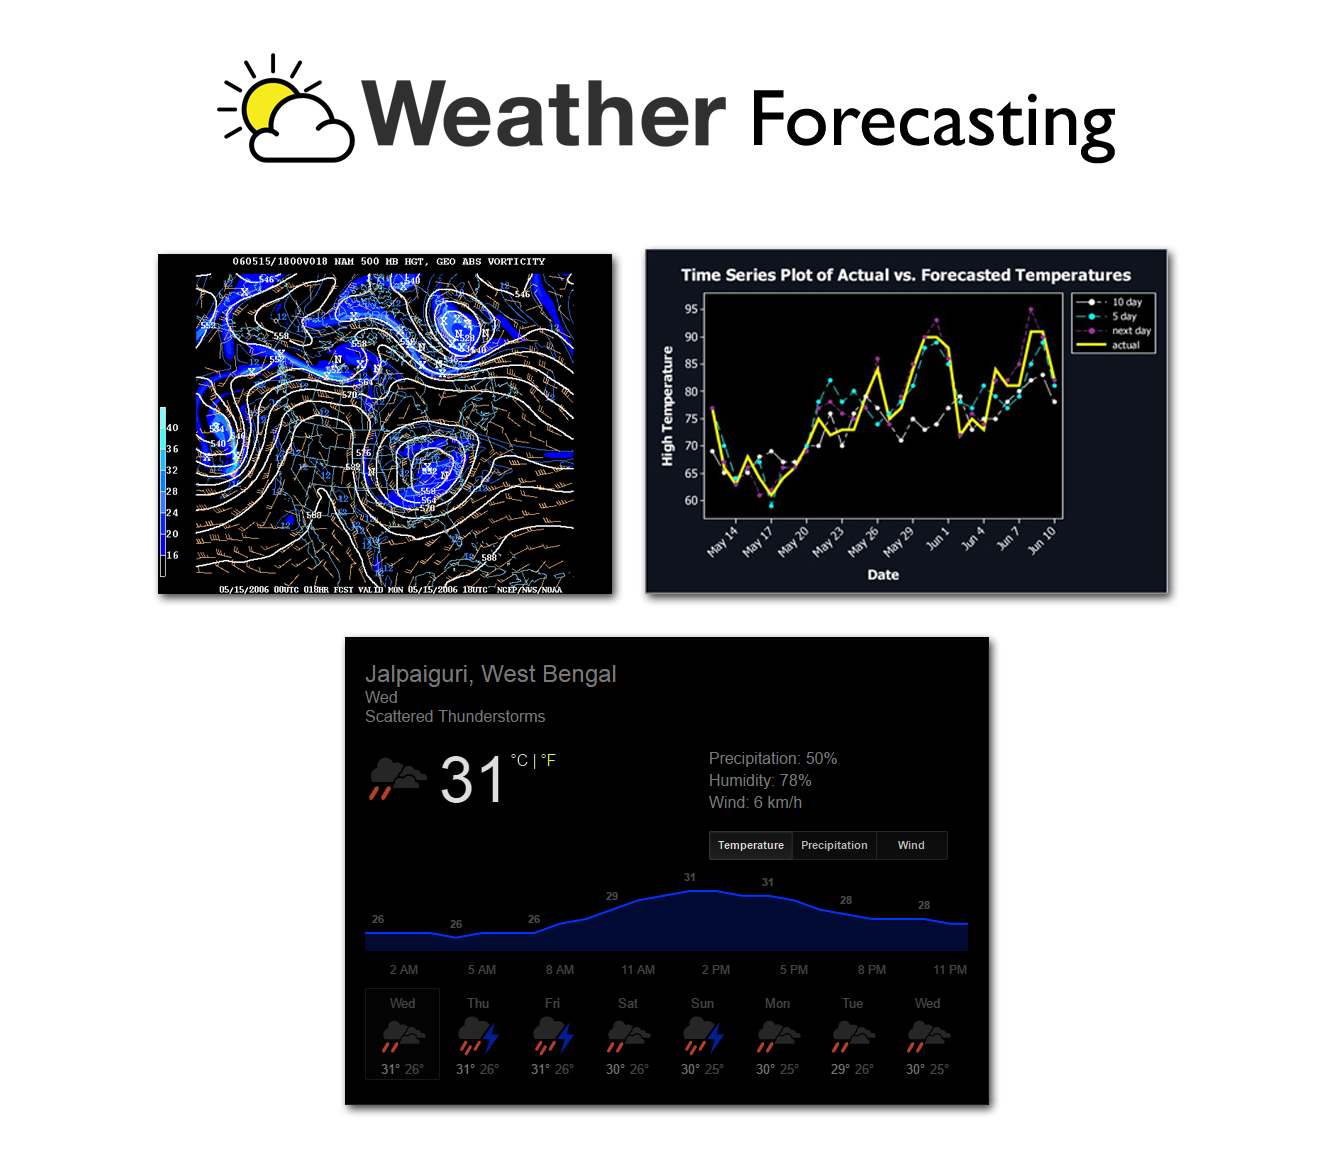
\includegraphics[scale=0.2]{images/wea}
		\end{center}
	\end{frame}
	
	\begin{frame}{Regression | Some Real Life Examples}
		\begin{figure}
			\begin{center}
				\vspace{-5mm}
				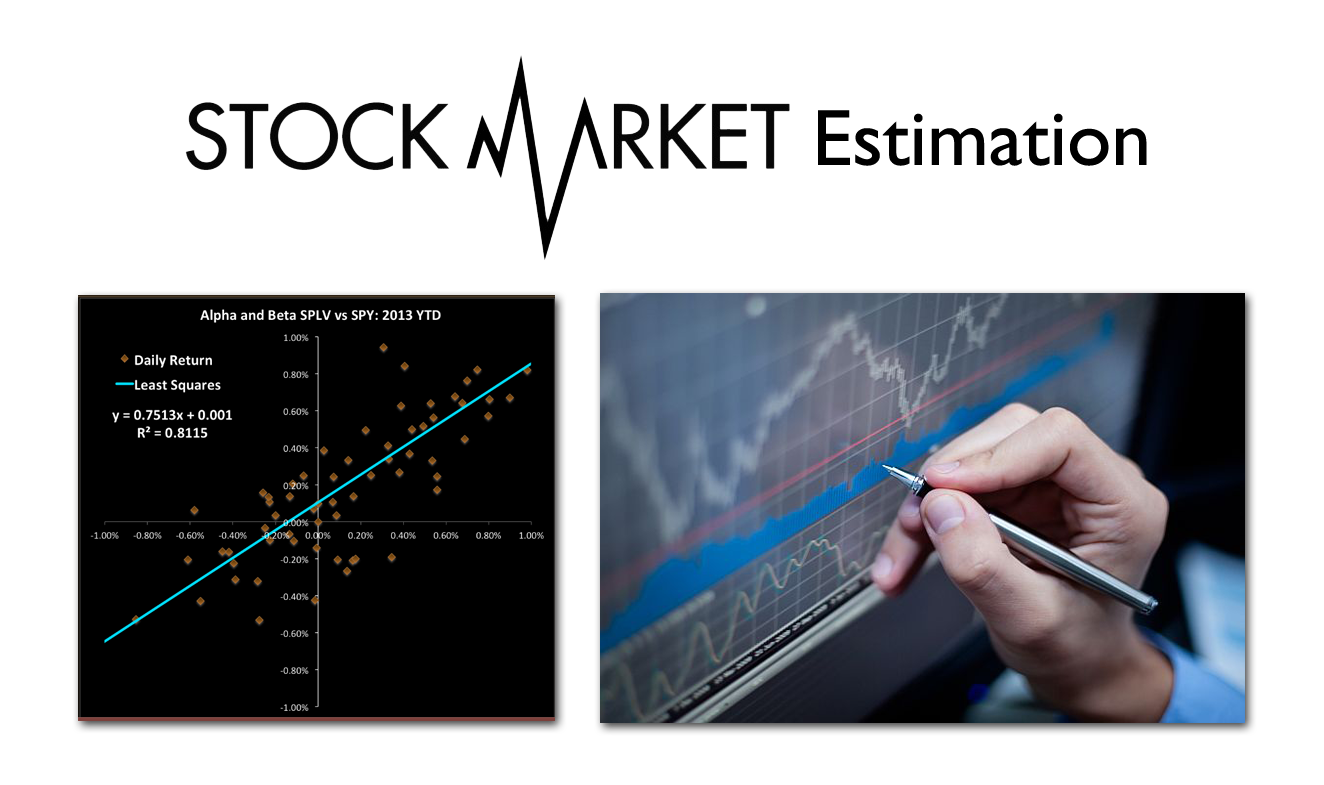
\includegraphics[scale=0.2]{images/sto}
				\caption{Stock Market Estimation}
			\end{center}
		\end{figure}
	\end{frame}
	
	\begin{frame}{Regression | Some Real Life Examples}
		\begin{figure}
			\begin{center}
				\vspace{-5mm}
				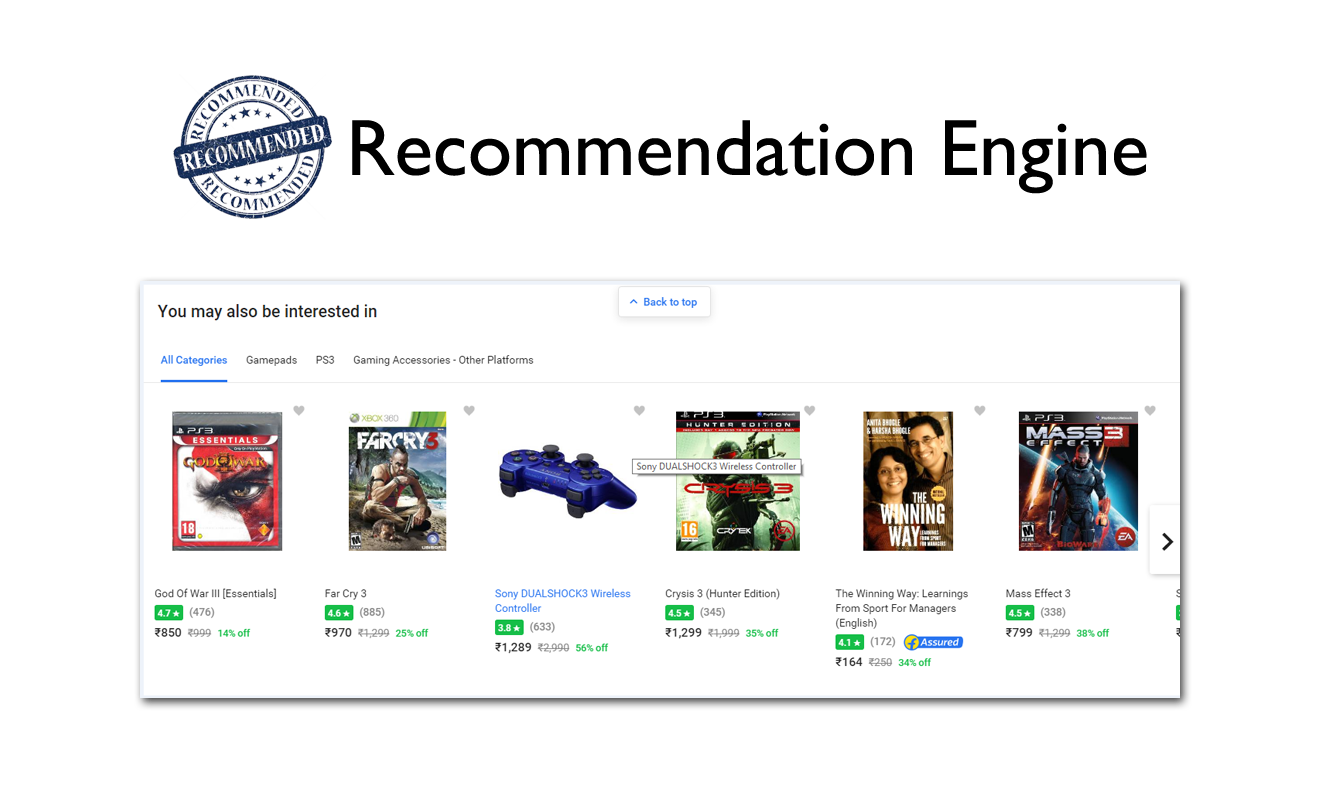
\includegraphics[scale=0.2]{images/reco}
				\caption{Recommendation Engine}
			\end{center}
		\end{figure}
	\end{frame}
	
	\begin{frame}{Regression | Some Real Life Examples}
		\begin{center}
			\vspace{-10mm}
			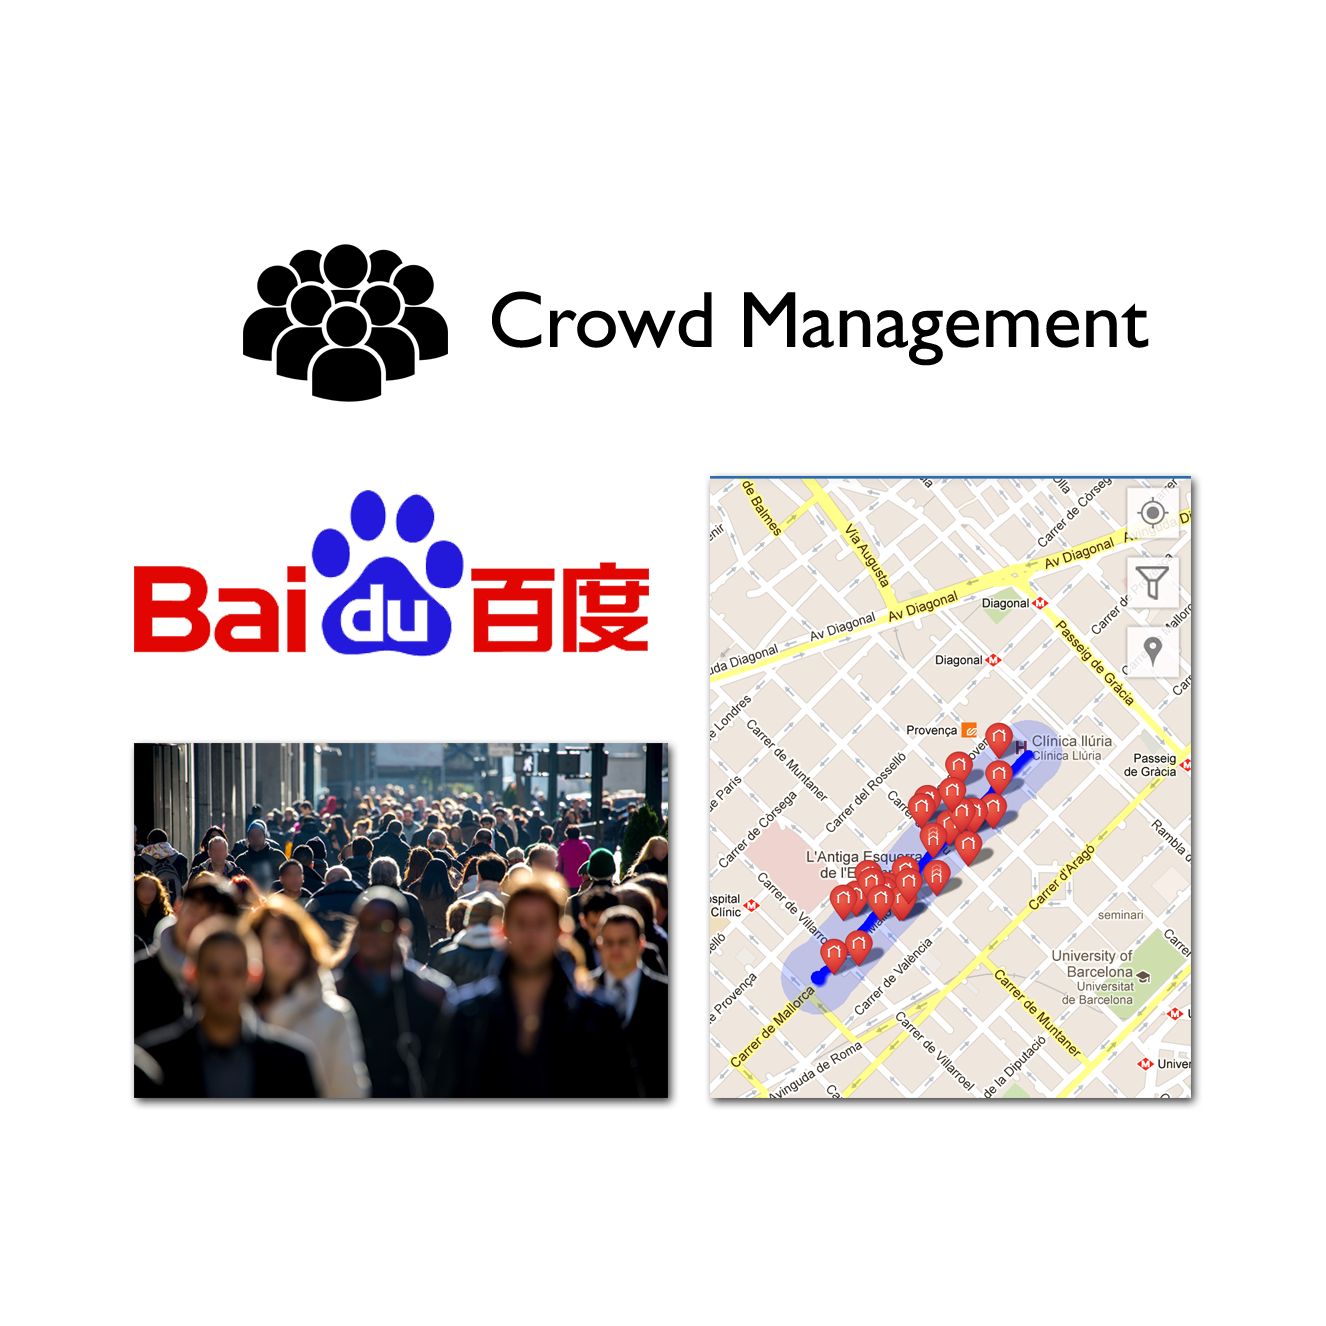
\includegraphics[scale=0.2]{images/crow}
		\end{center}
	\end{frame}
	
	\section{Classifications}
	\begin{frame}{Introduction | Classifications}
		\begin{center}
			\large{In machine learning and statistics, classification is the problem of identifying to which of a set of categories (sub-populations) a new observation belongs.}\\
			\bigskip
			\small{ On the basis of a training set of data containing observations (or instances) whose category 							membership is known.}
			\begin{figure}
				\centering
				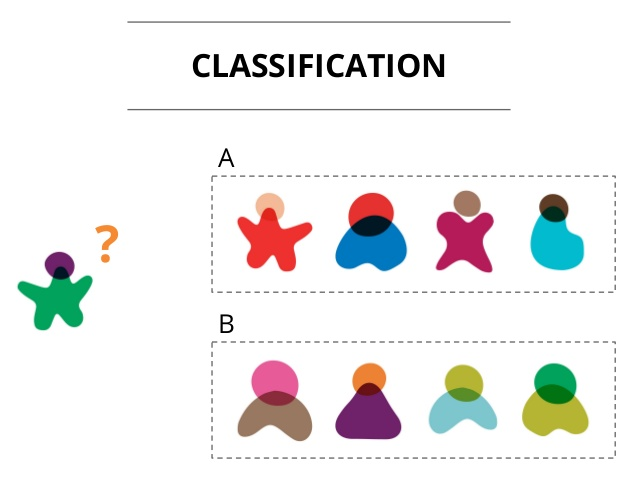
\includegraphics[width=60mm,height=40mm]{images/barun_1}
				\caption[]{Classification}
			\end{figure}
		\end{center}
		
	\end{frame}
	\subsection{Usages}
	\begin{frame}{Usages | When it is used?}
		\begin{center}
			\large{Classification is considered an instance of supervised learning, i.e. learning where a training set of correctly identified observations is available..}\\
			\bigskip
			
			\begin{figure}
				\centering
				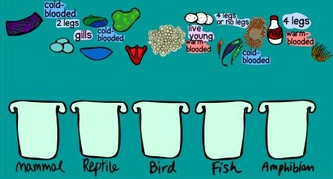
\includegraphics[width=60mm,height=40mm]{images/barun_2}
				\caption[]{Training set is correctly Identified.}
			\end{figure}
		\end{center}
	\end{frame}
	\begin{frame}{Usage | Types of Classifiers!!}
		\large{KNN algorithm :-}
		\begin{figure}
			\centering
			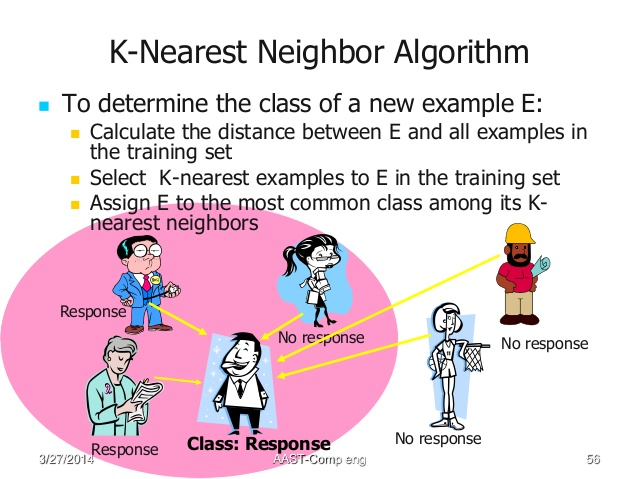
\includegraphics[width=70mm,height=60mm]{images/barun_3}
			\caption[]{Example}
		\end{figure}
	\end{frame}
	\begin{frame}{Usage | Types of Classifiers!!}
		\large{Decision Tree :-}\\
		\begin{figure}
			\centering
			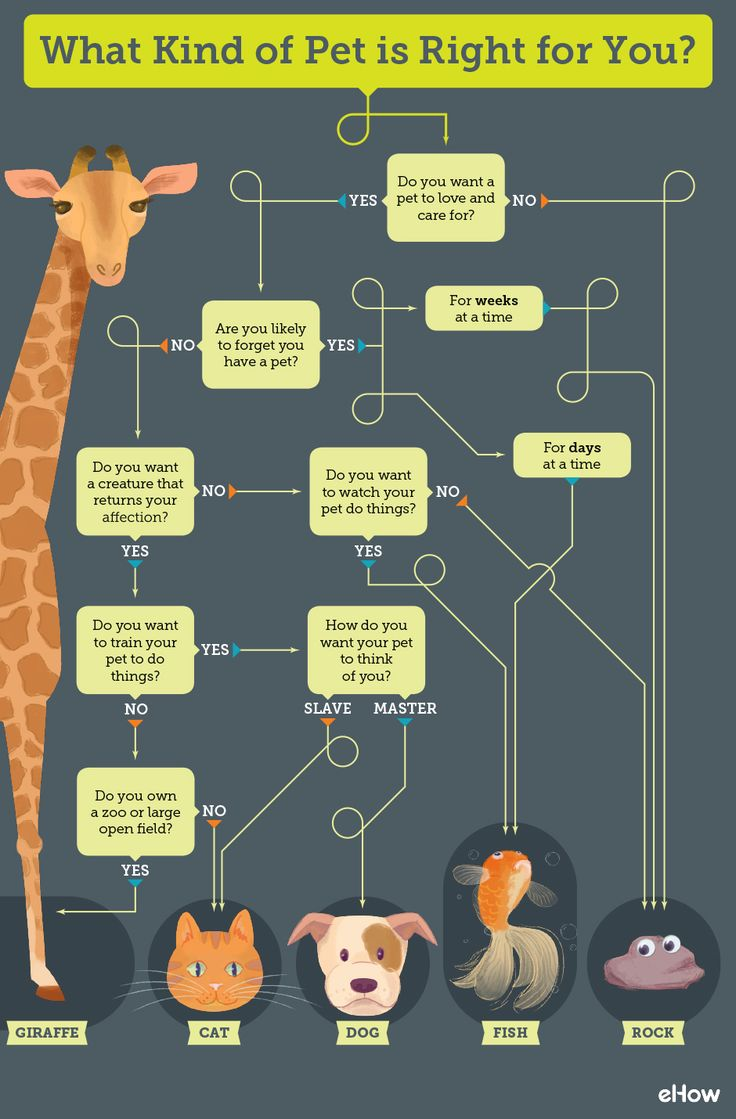
\includegraphics[scale=0.2]{images/barun_4}
			
		\end{figure}
	\end{frame}
	\subsection{Example Cases}
	\begin{frame}{Example Cases | Real Life Examples}
		\begin{center}
			
			\begin{itemize}
				\item<2-> Example 1:-
				An emergency room in a hospital measures 17 variables (e.g., blood pressure, age, etc) of newly admitted patients.
				A decision is needed: whether to put a new patient in an intensive-care unit.
				Due to the high cost of ICU, those patients who may survive less than a month are given higher priority.
				
				{\color{red} Problem: to predict high-risk patients and discriminate them from low-risk patients.}
				\item<3-> Example 2:-
				A credit card company receives thousands of applications for new cards. Each application contains information about an applicant,
				age
				Marital status
				annual salary
				outstanding debts
				credit rating
				etc.
				
				{\color{red}Problem: to decide whether an application should approved, or to classify applications into two categories, approved and not approved.}
			\end{itemize}
		\end{center}
	\end{frame}
	
	
	\section{Deep Learning}
	\begin{frame}{Deep Learning | What is Deep Learning}
		\centering{
			\movie[showcontrols=true]
			{           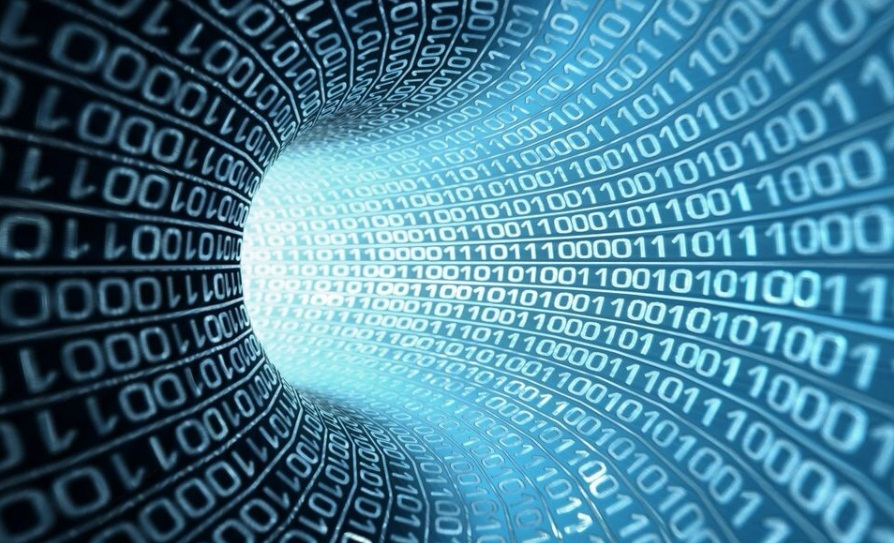
\includegraphics[scale=0.3 ]{images/somnath_4} } {video/somnath_5.mov}
		}
	\end{frame}
	\begin{frame}{Meaning | Deep Learning}
		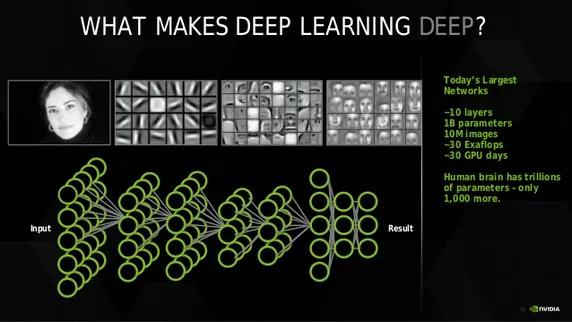
\includegraphics[scale=0.5]{images/somnath_1}
	\end{frame}
	\subsection{Neural Networks}
	\begin{frame}{Neural Networks | What is ANN?}
		\begin{figure}
			\centering
			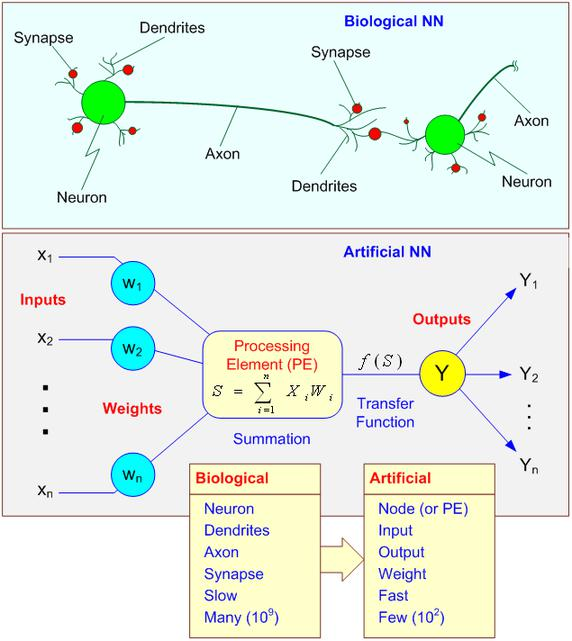
\includegraphics[width=60mm,height=70mm]{images/somnath_2}
			\caption[]{Artificial Neural Network}
		\end{figure}
	\end{frame}
	\subsection{Meaning}
	\begin{frame}{Traditional vs Deep learning | Deep Learning}
		\begin{figure}
			\centering
			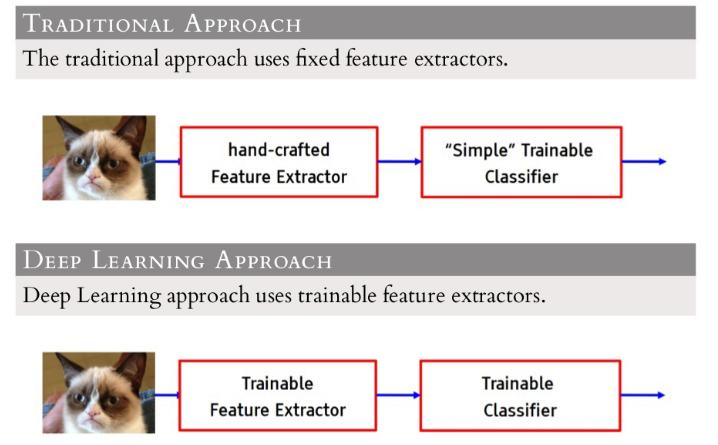
\includegraphics[width=80mm,height=70mm]{images/somnath_3}
			\caption[]{Tradition vs Deep Learning}
		\end{figure}
	\end{frame}
	
	\subsection{Advantages}
	\begin{frame}{Advantages | Deep Learning}
		\begin{center}
			\begin{itemize}
				\item Has best-in-class performance on problems that significantly outperforms other solutions in multiple domains. This includes speech, language, vision, playing games like Go etc. This isn’t by a little bit, but by a significant amount. The current record is from 2013 where it classified 9979 out of 10,000 images accurately. This performance is human equivalent or even better. A Silicon Valley–based startup called Vicarious claims it’s created an artificial intelligence program so advanced it can solve CAPTCHAs with accuracy that, in many cases, approaches 100 percent.
				\item Reduces the need for feature engineering, one of the most time-consuming parts of machine learning practice.
				
			\end{itemize}
			\begin{figure}
				\centering
				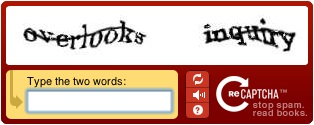
\includegraphics[width=30mm,height=10mm]{images/somnath_6}
				\caption[]{Captcha}
			\end{figure}
		\end{center}
	\end{frame}
	\subsection{Advantages}
	\begin{frame}{Disadvantages | Deep Learning}
		\begin{center}
			\begin{itemize}
				\item Requires a large amount of data — if you only have thousands of example, deep learning is unlikely to outperform other approaches.
				\item Is extremely computationally expensive to train. The most complex models take weeks to train using hundreds of machines equipped with expensive GPUs.
				\item Do not have much in the way of strong theoretical foundation. This leads to the next disadvantage.
				\item Determining the topology/flavor/training method/hyperparameters for deep learning is a black art with no theory to guide you.
				\item What is learned is not easy to comprehend. Other classifiers (e.g. decision trees, logistic regression etc) make it much easier to understand what’s going on.
				.
				
			\end{itemize}
		\end{center}
	\end{frame}
	\subsection{Usages}
	\begin{frame}{Usages | Deep Learning}
		\begin{center}
			
			
			Google Brain
			
			\centering{
				\movie[showcontrols=true]
				{                  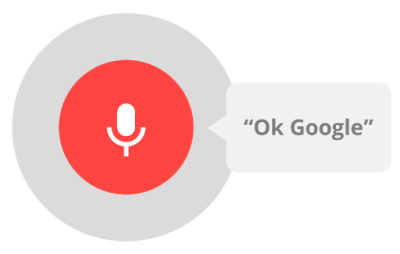
\includegraphics[scale=0.5]{images/somnath_11} } {video/somnath_10.mov}
			}
			
			
		\end{center}
	\end{frame}
	\begin{frame}{Usages | Deep Learning}
		\begin{center}
			
			
			GoogleDeepMind
			
			\centering{
				\movie[showcontrols=true]
				{                  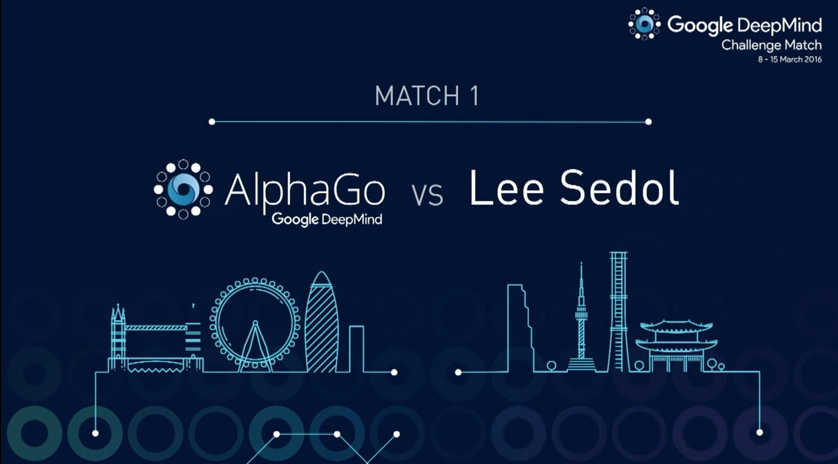
\includegraphics[scale=0.34]{images/somnath_9} } {video/somnath_12.mov}
			}
		\end{center}
	\end{frame}
	\begin{frame}{Usages | Deep Learning}
		\begin{center}
			
			
			Prisma
			
			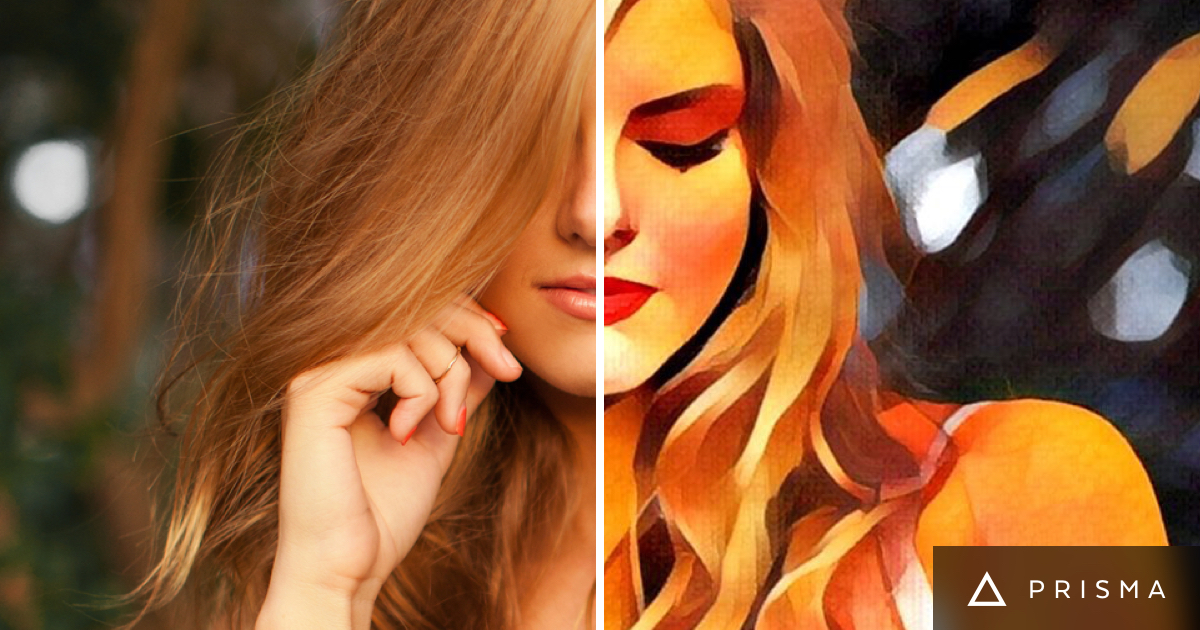
\includegraphics[scale=0.05 ]{images/somnath_13}
			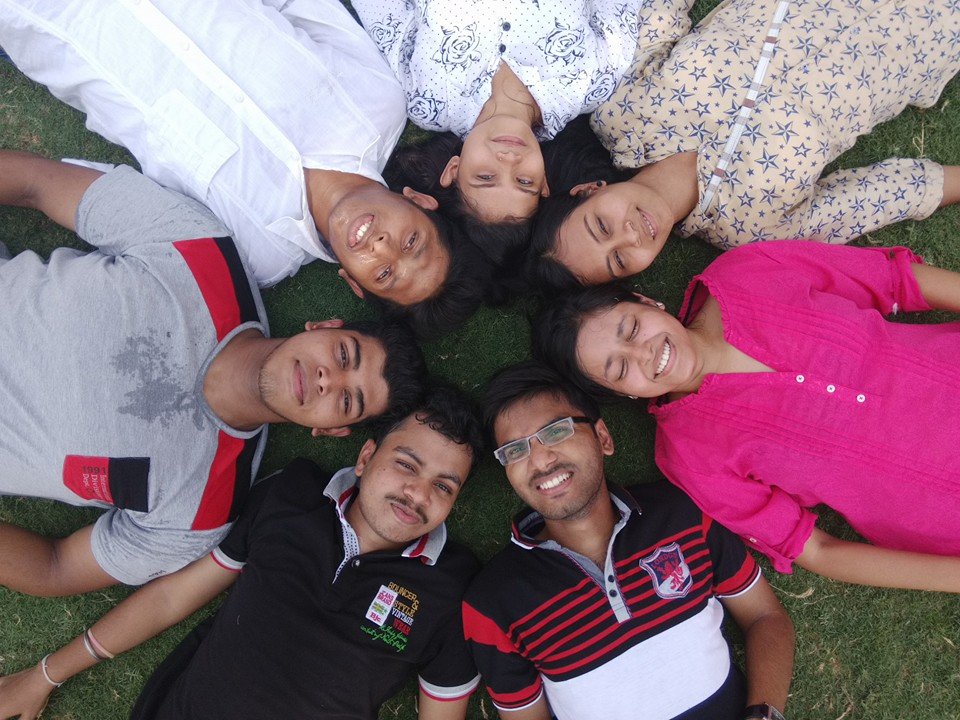
\includegraphics[width=40mm,height=40mm ]{images/somnath_14}  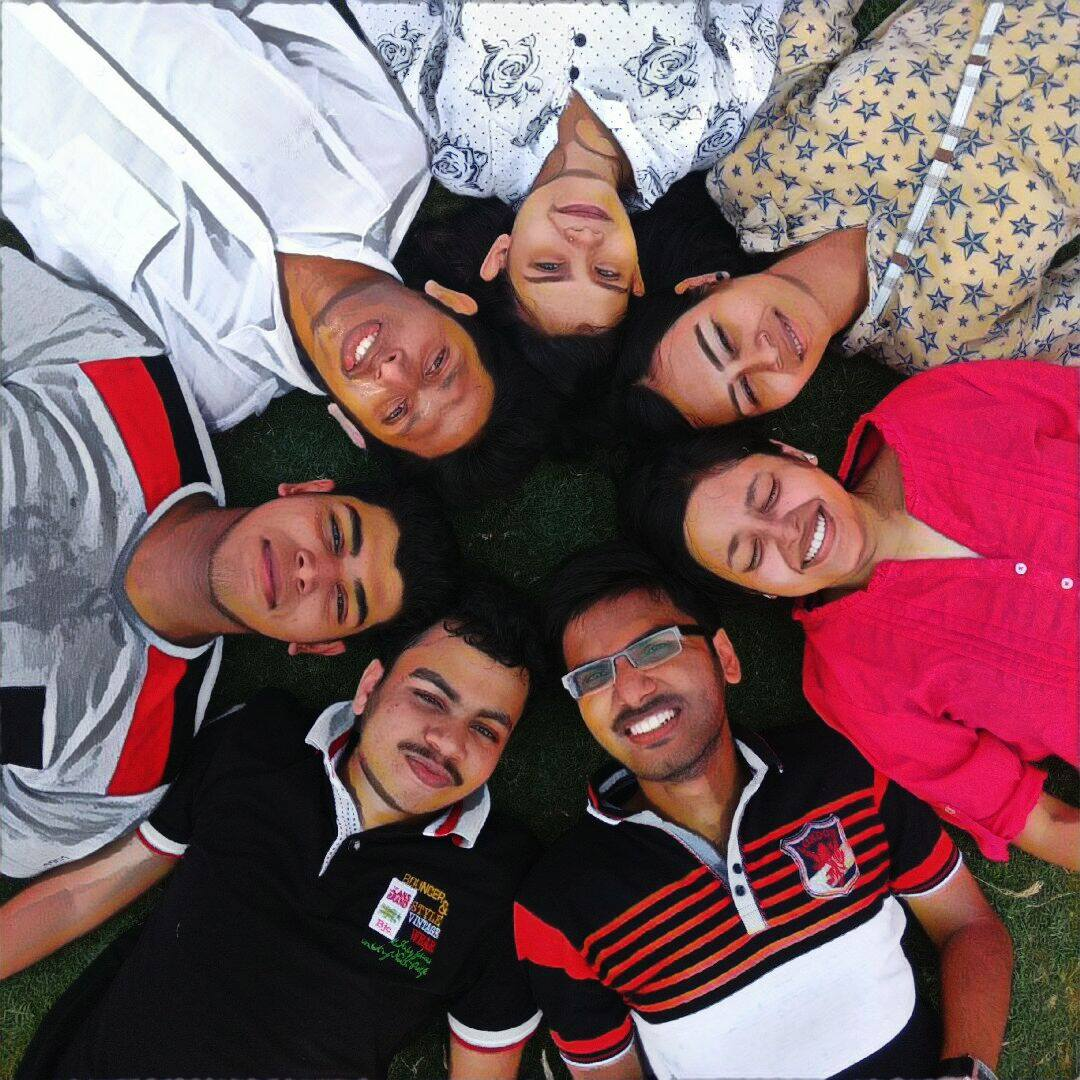
\includegraphics[width=40mm,height=40mm  ]{images/somnath_15}
			
			
		\end{center}
	\end{frame}
	\begin{frame}{Usages | Deep Learning}
		\begin{center}
			
			
			Mageta
			
			
			\centering{
				\movie[showcontrols=true]
				{                  
\includegraphics[scale=0.05 ]{images/somnath_8} } {video/somnath_7.mov}
			}
			
			
		\end{center}
	\end{frame}
	
	
	
	\section{Conclusion}
	\begin{frame}{Bibliography}
		\twocolumn
		\begin{itemize}
			\item \scriptsize{Phil Simon (March 18, 2013). Too Big to Ignore: The Business Case for Big Data. Wiley. p. 89. ISBN 978-1-118
				-63817-0.}
			\item \scriptsize{Mitchell, T. (1997). Machine Learning, McGraw Hill. ISBN 0-07-042807-7}
			\item \scriptsize{ Mehryar Mohri, Afshin Rostamizadeh, Ameet Talwalkar (2012) Foundations of Machine Learning, The MIT Press ISBN 9780262018258.}
			\item \scriptsize{Jordan, Michael I.; Bishop, Christopher M. (2004). "Neural Networks". In Allen B. Tucker. Computer Science Handbook, Second Edition (Section VII: Intelligent Systems). Boca Raton, FL: Chapman \& Hall/CRC Press LLC. ISBN 1-58488-360-X.}
			\item \scriptsize{https: //www.kaggle.com/c/twitter-psychopathy-prediction}
			\item \scriptsize{Mastering the game of Go with deep neural networks and tree search (2016), D. Silver et al.}
		\end{itemize}
		\onecolumn
	\end{frame}
	\endgroup
	
	\begingroup
	\setbeamercolor{background canvas}{bg=blue_dark}
	\setbeamercolor{normal text}{fg=blue_light}
	\begin{frame}[plain,c]
		\hspace*{6 mm}
		\vspace*{-18 mm}
		\textcolor{blue_light}{\Large{Now that was very interesting!}}
	\end{frame}
	\begin{frame}[plain,c]
		\hspace*{27 mm}
		\vspace*{-20 mm}
		\textcolor{blue_light}{\Large{The End}}
	\end{frame}
	\endgroup
	
\end{document}
